%!TEX root = ../Thesis.tex
\chapter{Decoupling Feature Extraction and Classification Layers for Calibrated Neural Networks}
\label{chap:ICML}
In this Chapter, I present our ICML paper "Decoupling Feature Extraction and Classification Layers for Calibrated Neural Networks". As mentioned in the introduction of the thesis, this work actually started somewhere else entirely. This project started because Professor Olmos had recently been working on methods for robustness against adversarial attack and we were interested in developing generative classifiers with the hope that they would be robust to such attacks. We were not the first to consider this idea. Back in the early 2000s \cite{NIPS2001_7b7a53e2} started arguing that perhaps generative classifiers had benefits over discriminative ones, and in \cite{Schott2018TowardsTF} and \cite{li2019are} the authors looked at specifically using latent variable models for robustness against adversarial attacks. We had similar ideas but specified different variational families that could encompass pre-trained models (the exact form of these is not interesting for this thesis). Unfortunately, training these models was extremely unstable using the ELBO, due to similar reasons as those mentioned in \cite{fetaya2020understanding}, meaning we obtained very poor accuracy on the test set. I therefore chose to train the model only with cross-entropy to start with, and after converging on cross-entropy, I would "turn-on" the ELBO loss whilst freezing the backbone parameters of the encoder model - unfortunately to no avail. We saw no improvements in adversarial robustness. \\

\noindent Around Christmas time I was desperate as the ICML deadline was approaching and we had no good results. I suggested to Professor Olmos that perhaps we should just try to evaluate the models using the typical calibration metrics also used in BNN evaluations, and lo and behold: the calibration metrics were (in my opinion) extremely good - better than many other model types I had used before on CIFAR-10 and CIFAR-100. These metrics were still obtained using the latent variable model we had proposed (essentially a classical variational auto-encoder (VAE) \citep{kingma2014vae} where the decoder is replaced with an MLP that performs classification based on the latent variable $\mathbf{z}$), but with the twist that it was first trained only using cross-entropy, \textit{after which several of the first layers of the encoder were frozen and the decoder was re-initialized} and then trained with ELBO (reading the paper, this exact setup will become clearer - this is what we later named V-TST). As we were unsure of whether it was the latent variable model or the other training steps (i.e. re-initialising the final layers and freezing the first layers) were the main driver of the improvement in calibration, we ran a number of ablation experiments, including one where we still trained in two stages, but using cross-entropy in both (i..e no latent variable model). Once again we were extremely surprised to see that the models trained in this way were extremely well calibrated on in-distribution and shifted data - only at the cost of a few additional epochs of training (this is what we named TST in the paper). As we did not have any good theoretical explanations for this behaviour we ran a large number of experiments and ablation studies to validify these findings, and found them to hold across several different datasets and architecture, and thus the ICML paper was born. \\

\noindent I write about this story here because it, to me, is so paradoxical, that the paper I have written where the performance gains are perhaps the largest, is also the paper which perhaps is the least principled, was the least planned and methodologically the simplest. It is to me the epitome of what it means to write a PhD and doing research - few things go as planned, but sometimes rolling with the punches and pushing on will lead to some unplanned discovery. \\

\noindent To return to the paper: the contributions of this paper can be summarized as two methods for training calibrated neural networks for classification, Two-Stage Training (TST) and Variational Two-Stage Training (V-TST). In TST any neural network model is trained using cross-entropy end-to-end until early stopped or converged (Stage 1), after which the feature extraction layers of the network are frozen and the final layers (could just be the logits layer) is re-initialized and trained using cross-entropy until early-stopped based on validation loss (Stage 2). In V-TST, Stage 1 is identical to that of TST, but in Stage 2 a latent variable is additionally introduced in the final layers of the network\footnote{This model is essentially a VAE where the decoder is replaced with an MLP, and the ELBO loss consists of the negative log-likelihood loss of the class $y$ and KL divergence between the variational distribution $q(\mathbf{z}|\mathbf{x})$ and prior $p(\mathbf{z})$.} and the model is trained with the ELBO loss (but once again early-stopped based on cross-entropy validation loss). We show that these methods lead to better calibrated neural networks on several datasets and architectures, and also showcase when they do not work.\\

\noindent At the time we tried to explain why these methods work from a perspective of the feature-embedding space, but since then we have had different thoughts and ideas for why this might be the case. Firstly, Professor Morten Mørup from DTU recently brought up an interesting explanation for TST working as well as it does. Morten reminded me of the connection between early-stopping and cross-validating L2 regularization, and mentioned that the TST method may in fact just be finding the perfect regularization for a learnt feature extractor thus explaining the calibration improvements - this would also explain why TST does not improve out-of-distribution metrics. Secondly, an interesting motivation for why V-TST at times further improves calibration metrics in comparison to TST, may be because the sampling of $\mathbf{z}$ at training time can be seen as self-learnt data augmentation (this idea was largely inspired by \cite{Trinh2022TacklingCS}). To be specific, the sampled $\mathbf{z} \sim \mathcal{N}(\mu_{\beta, \theta}(\mathbf{x}), \sigma_{\beta, \theta}(\mathbf{x}))$ can be mapped back into the $\mathcal{X}$ space by some perturbation specified by the variational posterior $q(\mathbf{z}|\mathbf{x})$. We have not further pursued or investigated these ideas, but find that they may provide interesting insights into why TST and V-TST works.

\noindent 



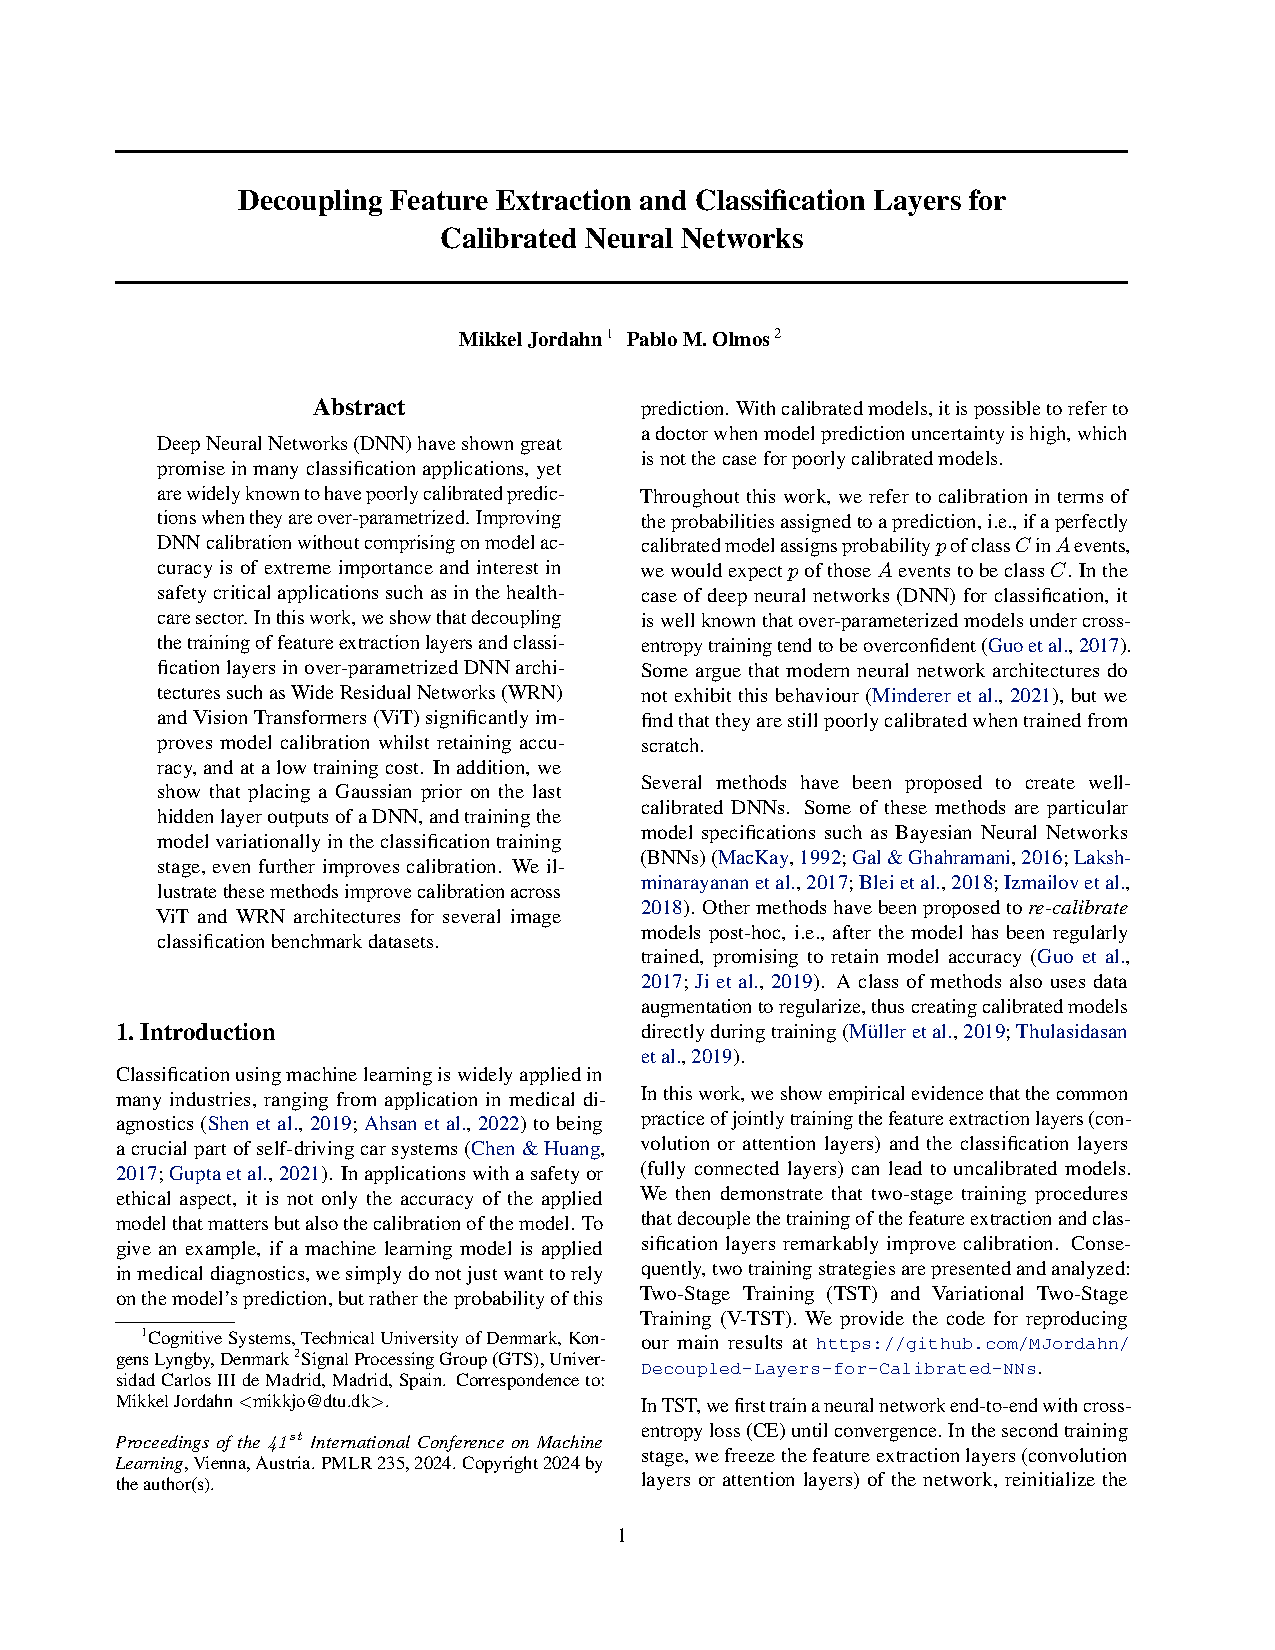
\includepdf[pages=-, offset=0mm 0mm, delta=0mm 0mm, scale=1.0, pagecommand={\thispagestyle{mystuff}{}{}{}}]{chapters/paperA_TST/TST.pdf}